\documentclass[10pt,a4paper]{article}
\usepackage[latin1]{inputenc}
\usepackage{amsmath}
\usepackage{amsfonts}
\usepackage{amssymb}
\usepackage{fullpage}
\usepackage{graphicx}

\begin{document}
\title{J.D. Jackson Problem 4.1}
\author{Josh Orndorff \\ admin@joshorndorff.com}
\maketitle

\section{Charges in the $xy$--plane}
The first step here is to write the charge distribution $\rho$ in spherical coordinates.  I'll first write $\rho_1$, the charge distribution of the single point charge on the positive x-axis.  We know that the distribution will contain several delta functions and be proportional to q.
\begin{equation}
\rho_1 = Aq\delta(r-a)\delta(\theta-\frac{\pi}{2})\delta(\phi)
\end{equation}

To find the proportionality constant, A, we will integrate both sides over all space knowing that the total integral is equal to the charge, q.
\begin{equation}
q = \int_0^{2\pi}\int_0^\pi\int_0^\infty A q \delta(r-a)\delta(\theta-\frac{\pi}{2})\delta(\phi) r^2 \sin\theta \,\mathrm{d}r\,\mathrm{d}\theta\,\mathrm{d}\phi
\end{equation}
\begin{equation}
1 = \int_0^\pi A \delta(\theta-\frac{\pi}{2}) \sin\theta \,\mathrm{d}\theta
\end{equation}
\begin{equation}
A=\frac{1}{2\pi a^2}
\end{equation}
Plugging this back in, we get the final form of this charge distribution.
\begin{equation}
\rho_1 = \frac{q}{2\pi a^2} \delta(r-a)\delta(\theta-\frac{\pi}{2})\delta(\phi)
\end{equation}

Note that it would be just as acceptable, and more general, to use $A=\frac{1}{2\pi r^2}$ as the delta functions would pick out the correct values of $r$ upon integration.  Using the more general form which includes $r$ rather than $a$ will also solve the problem if a charge is placed at the origin (i.e, $r=0$).  I mention this here because we will rely on this logic to handle the $\theta$ dependence in the next section.
We can now proceed to write the total charge distribution due to all four point charges.
\begin{equation}
\rho = \frac{q}{2\pi a^2} \delta(r-a)\delta(\theta-\frac{\pi}{2})\left[\delta(\phi)+\delta(\phi-\frac{\pi}{2})-\delta(\phi-\pi)-\delta(\phi-\frac{3\pi}{2})\right]
\end{equation}

We can calculate the $q_{lm}$'s by applying equation 4.3 from Jackson to calculate, $q_{lm}=\int Y_{lm}^* r^l \rho \mathrm{d}V$.
\begin{equation}
q_{lm} = \frac{q}{2\pi a^2} \int_0^{2\pi}\int_0^\pi\int_0^\infty
Y_{lm}^*(\theta, \phi)r^{l+2}\delta(r-a)\delta(\theta-\frac{\pi}{2})\left[\delta(\phi)+\delta(\phi-\frac{\pi}{2})-\delta(\phi-\pi)-\delta(\phi-\frac{3\pi}{2})\right]
\sin\theta \mathrm{d}r\mathrm{d}\theta\mathrm{d}\phi
\end{equation}

After evaluating the r integral,
\begin{equation}
q_{lm} = \frac{qa^l}{2\pi} \int_0^{2\pi}\int_0^\pi
Y_{lm}^*(\theta, \phi)\delta(\theta-\frac{\pi}{2})\left[\delta(\phi)+\delta(\phi-\frac{\pi}{2})-\delta(\phi-\pi)-\delta(\phi-\frac{3\pi}{2})\right]
\sin\theta \mathrm{d}\theta\mathrm{d}\phi
\end{equation}

After evaluating the $\theta$ integral,
\begin{equation}
q_{lm} = \frac{qa^l}{2\pi} \int_0^{2\pi}
Y_{lm}^*(\frac{\pi}{2}, \phi)\left[\delta(\phi)+\delta(\phi-\frac{\pi}{2})-\delta(\phi-\pi)-\delta(\phi-\frac{3\pi}{2})\right]
\mathrm{d}\phi
\end{equation}

After evaluating the $\phi$ integral,
\begin{equation}
q_{lm} = \frac{qa^l}{2\pi} \left[Y_{lm}^*(\frac{\pi}{2}, 0)+Y_{lm}^*(\frac{\pi}{2}, \frac{\pi}{2})-Y_{lm}^*(\frac{\pi}{2}, \pi)-Y_{lm}^*(\frac{\pi}{2}, \frac{3\pi}{2})\right]
\end{equation}

Technically that does it, but we can go a little further and simplify those $Y_{lm}^*$'s using equation 3.53 in Jackson.
After evaluating the $\phi$ integral,
\begin{equation}
q_{lm} = \frac{qa^l}{2\pi} \sqrt{\frac{2l+1}{4\pi}\frac{(l-m)!}{(l+m)!}}P_l^m(\cos\frac{\pi}{2})
\left[e^{-im0} + e^{-im\frac{\pi}{2}} - e^{-im\pi} - e^{-im\frac{3\pi}{2}}\right]
\end{equation}

\begin{equation}
q_{lm} = \frac{qa^l}{2\pi} \sqrt{\frac{2l+1}{4\pi}\frac{(l-m)!}{(l+m)!}}P_l^m(0)
\left[1 + \left(e^{-i\frac{\pi}{2}}\right)^m - \left(e^{-i\pi}\right)^m - \left(e^{-i\frac{3\pi}{2}}\right)^m\right]
\end{equation}

\begin{equation}
q_{lm} = \frac{qa^l}{2\pi} \sqrt{\frac{2l+1}{4\pi}\frac{(l-m)!}{(l+m)!}}P_l^m(0)
\left[1 + (-i)^m - (-1)^m - (i)^m\right]
\end{equation}

Considering only the portion in brackets, we see that the $q_{lm}$'s are non-zero only when m is odd, and that allows further simplification.
\begin{equation}\boxed{
q_{lm} = \frac{qa^l}{\pi} \sqrt{\frac{2l+1}{4\pi}\frac{(l-m)!}{(l+m)!}}(1-i^m)P_l^m(0)
}\end{equation}

\begin{subequations}
The first few $q_{lm}$'s are,
\begin{align}
        q_{1,1}&=\frac{-qa}{2\pi}\sqrt{\frac{3}{2\pi}}(1-i) \\
        q_{1,-1}&=\frac{qa}{2\pi}\sqrt{\frac{3}{2\pi}}(1+i)
\end{align}
\end{subequations}

\section{Charges on the $z$--axis}
As mentioned above, the charge distribution can be written with an $r^2$ and by the same logic $\sin \theta$ in the denominator.  This troubled me at first, but integrating such a charge distribution over \textit{any} region results in the correct total charge.
\begin{equation}
\rho=\frac{q}{2\pi\sin\theta r^2}\left[\delta(r-a)\left(\delta(\theta)+\delta(\theta-\pi)\right)-2\delta(r)\right]
\end{equation}

\begin{equation}
q_{lm}=\frac{q}{2\pi}
\int_0^{2\pi}\int_0^\pi\int_0^\infty Y_{lm}^*(\theta,\phi) r^l
\left[\delta(r-a)\left(\delta(\theta)+\delta(\theta-\pi)\right)-2\delta(r)\right]
\mathrm{d}r \mathrm{d}\theta \mathrm{d}\phi
\end{equation}

In this case, we know that $m=0$ because of azimuthal symmetry so the spherical harmonics simplify.
\begin{equation}
q_{l0}=\frac{q}{2\pi}\sqrt{\frac{2l+1}{4\pi}}
\int_0^{2\pi}\int_0^\pi\int_0^\infty P_l(\cos\theta) r^l
\left[\delta(r-a)\left(\delta(\theta)+\delta(\theta-\pi)\right)-2\delta(r)\right]
\mathrm{d}r \mathrm{d}\theta \mathrm{d}\phi
\end{equation}

Evaluating the integrals is relatively straight-forward, except for that last delta in the case of $l=0$.  In this case, $r^l=0^0$ which is undefined in general.  However, Jackson lists the proper value to use as equation 4.4.
\begin{equation}
q_{l0}=qa^l\sqrt{\frac{2l+1}{4\pi}}
[P_l(\cos0) + P_l(\cos\pi)]-\frac{2q}{\sqrt{4\pi}}\delta_{l,0}
\end{equation}
\begin{equation}
q_{l0}=qa^l\sqrt{\frac{2l+1}{4\pi}}
[1 + (-1)^l]-\frac{2q}{\sqrt{4\pi}}\delta_{l,0}
\end{equation}

As before, examining the bracketed part of the equation shows that only even $l$'s result in non-zero $q_l0$'s.  When $l$ is even,
\begin{equation}
q_{l0}=2qa^l\sqrt{\frac{2l+1}{4\pi}}-\frac{2q}{\sqrt{4\pi}}\delta_{l,0}
\end{equation}

\begin{equation}\boxed{
q_{l0}=\frac{2q}{\sqrt{4\pi}}(a^l\sqrt{2l+1}-\delta_{l,0})
}\end{equation}

\begin{subequations}
The first few non-zero $q_l0$'s are,
\begin{align}
        q_{2,0}&=qa^2 \sqrt{\frac{5}{\pi}} \\
        q_{4,0}&=qa^4\sqrt{\frac{9}{\pi}}
\end{align}
\end{subequations}

\section{Multipole expansion for electric potential}
The proper expansion is given as equation 4.1 in the text.  Substituting the form for $q_l0$ that we just found and simplifying the $Y_{lm}$ for $m=0$ gives,
\begin{equation}
\Phi=\frac{1}{4\pi\epsilon_0}\sum_l\frac{4\pi}{2l+1}
\left[\frac{2q}{\sqrt{4\pi}}(a^l\sqrt{2l+1}-\delta_{l,0})\right]
\sqrt{\frac{2l+1}{4\pi}}P_l(\cos\theta)
\end{equation}
\begin{equation}
\Phi=\frac{2q}{4\pi\epsilon_0}\sum_l
(a^l-\delta_{l,0})P_l(\cos\theta)
\end{equation}

The lowest non-zero term is the $l=2$ term, so in the $xy$--plane,
\begin{equation}
\Phi_2(r)=\frac{qa^2}{4\pi\epsilon_0 r^3} \qquad
\Phi_2(a)=\frac{q}{4\pi\epsilon_0 a} \qquad
\lim_{r\rightarrow\infty}\Phi_2(r)=0
\end{equation}

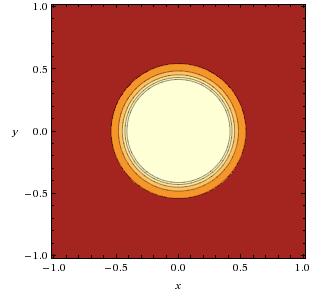
\includegraphics{a.png} 

\section{Exact calculation of electric potential}
Calculating the exact potential from Coulomb's law for this potential is actually quite a bit easier.  I'll do the calculation for the negative charge and then for one of the positive charges.

\begin{equation}
\Phi_-=\frac{-2q}{4\pi\epsilon_0r}
\end{equation}
\begin{equation}
\Phi_+=\frac{q}{4\pi\epsilon_0\sqrt{a^2+r^2}}
\end{equation}
\begin{equation}
\Phi_{total}=\Phi_- + 2 \Phi_+ = \frac{q}{2 \pi \epsilon_0} \left( \frac{1}{\sqrt{a^2+r^2}}-\frac{1}{r}\right)
\end{equation}

\end{document}